%----------------------------------------------------------------------------------------
%	PACKAGES AND DOCUMENT CONFIGURATIONS
%----------------------------------------------------------------------------------------

\documentclass[10pt,a4paper]{scrartcl}

% Adjusting margins to personal my need
\addtolength{\oddsidemargin}{-.5in}
\addtolength{\evensidemargin}{-.5in}
\addtolength{\textwidth}{1in}
\addtolength{\topmargin}{-.5in}
\addtolength{\textheight}{1in}

% Graphics
\usepackage{caption}
\usepackage{graphicx}
\graphicspath{{figures/}}

% Math
\usepackage{amssymb}
\usepackage{amsmath} % Required for some math elements 
\usepackage{amsthm}
\usepackage{mathtools}

% Other
\usepackage{algorithmic}
\usepackage{array}
\usepackage{lipsum}
\usepackage{hyperref}

\usepackage{algorithm}
\usepackage{algorithmic}

\usepackage{enumitem}
\usepackage[
    backend=biber,
    style=alphabetic,
]{biblatex}

\usepackage{tikz}
\usepackage{circuitikz}
\usetikzlibrary{arrows,shapes,positioning}
\usepackage{subfig}
\usepackage{xcolor}

\usepackage{booktabs}


\usetikzlibrary{shadings} % LaTeX and plain TeX when using TikZ



\addbibresource{bibliography/sample.bib}

\captionsetup[figure]{
%  font = it,
  labelfont = it
}

\setlength{\tabcolsep}{0pt}

\newtheorem{theorem}{Theorem}
\newtheorem{conjecture}{Conjecture}
\newtheorem*{remark}{Remark}
\newtheorem{corollary}{Corollary}[theorem]


% \captionsetup[table]{
% %  font = it,
%   labelfont = it
% }

\definecolor{perfect-color}{HTML}{228B22}


%----------------------------------------------------------------------------------------
%	MAIN PART
%----------------------------------------------------------------------------------------
\begin{document}
\title{\Large ACubed: A Machine Learning Approach to Enhance Skill Measurement in Rhythm Games}
%\subtitle{Proposal to Improve Difficulty, AAA Equivalency, and Skill Rating Formulas}
\author{\large Wilson Cheung (WirryWoo)\\
\normalsize \textit{Georgia Institute of Technology}}
\date{\vspace{-3ex}}

\maketitle % Inserts the title, author and date




%----------------------------------------------------------------------------------------
%	Abstract
%----------------------------------------------------------------------------------------
\begin{abstract}
	\normalsize
	%% Text of the abstract
	\textbf{Abstract:} The objective of this study is to explore methods to improve the scalability and standardization of skill-based metrics in Flash Flash Revolution (FFR). For stepfile difficulty, we propose an ensemble model that combines tree-based methods with a time series extrinsic regression model to capture local and global patterns in stepfiles using objectively defined time-sensitive features. Additionally, we introduce a framework that utilizes the expectation-maximization algorithm to determine a player's AAA equivalency rating and overall skill rating, providing a quantitative measure of their skill. These models can be optimized for training and evaluation through the use of ACubed, a Python module that incorporates a machine learning framework for updating the underlying formula of skill-based metrics, with the ultimate goal of improving the overall competitive experience for FFR players.
\end{abstract}

%----------------------------------------------------------------------------------------
%	Table of Content
%----------------------------------------------------------------------------------------
\setcounter{tocdepth}{2}
\tableofcontents


\clearpage

%----------------------------------------------------------------------------------------
%	Main Part
%----------------------------------------------------------------------------------------
\section{Introduction and Motivation}
\label{sec:introduction}

\href{https://www.Flash Flash Revolution.com/}{Flash Flash Revolution} (FFR) is a renowned Flash-based vertical scrolling rhythm game that was originally developed by \texttt{Synthlight} in 2002. Similar to its predecessor Dance Dance Revolution (DDR), players are presented with a sequence of arrows, referred to as \textit{stepfiles}, which are meticulously calibrated and synchronized to the background music. The main objective is to maximize the raw score by pressing the corresponding keys within a precise timing window of less than one-quarter of a second, ensuring a perfect alignment between the arrows in motion and the static receptors. Following the deprecation of Adobe Flash Player in 2020, FFR is now accessible through RCubed, an open-source engine developed and actively maintained by \texttt{Velocity} \cite{20200427}.

\vspace{2mm}

The player base of FFR maintains a consistently robust presence, with several thousand users actively engaging in gameplay every month. Among this devoted community are competitive players hailing from online rhythm games such as osu!mania and Etterna, with a notable number participating in official tournaments each year. To ensure a positive experience for these players, many systems have been created to objectively measure stepfile difficulty, fairly reward scores based on playing performance, and determine ratings that accurately reflect the player's skill. Although these systems are widely adopted in the community, their design has sparked considerable concerns regarding the reliability and scalability of their skill measurement.

\vspace{2mm}

Before delving into these areas of discussion, it is important to acknowledge that there will be many assumptions present throughout this analysis. We will provide sufficient justification for any assumptions made, and it is important to note that the proposed solutions in this paper are not absolute and definitive. If there is any disagreement with any identified assumptions, it is encouraged for individuals to develop an alternative modeling approach based on their preferred assumptions.

\subsection{Overview of FFR's Skill-Based Metrics and Their Shortcomings}
\subsubsection{Stepfile Difficulty}
Every stepfile possesses intrinsic levels of challenge concerning the player's execution due to their distinct structural characteristics. However, quantifying this measure continues to be a challenging question. In the initial stages of its development, the measurement of stepfile difficulty in FFR was based on a scale ranging from \texttt{1} to \texttt{12}, where \texttt{1} represented the easiest and \texttt{12} represented the most difficult level. However, in 2012, \texttt{nois-or-e}, \texttt{One Winged Angel}, and \texttt{stavie33} improved upon this method by introducing a more granular scale ranging from \texttt{1} to \texttt{120}. This update was announced on the forums \cite{20120608} and has since been adopted as the current difficulty scale in use.

\vspace{2mm}

To assess the difficulty of new stepfiles in the engine, a team of difficulty consultants within the community assigns a numerical rating on an integer scale of \texttt{1} to \texttt{120}, taking into consideration factors such as feedback from other players and the level of challenge posed by existing stepfiles of similar difficulty ratings. However, this process raises the following concerns:
\begin{itemize}
	\item By solely relying on pairwise stepfile comparisons to determine the difficulty rating of an unrated stepfile, other assigned ratings are not considered during comparison, resulting in an inconsistent set of criteria established across stepfiles to define difficulty.
	\item Proposed difficulty ratings crowdsourced from the vocal minority are inherently subject to self-selection bias by the current process's mechanism design. Moreover, manual stepfile difficulty assignment for easier files is generally less accurate due to higher skill bias in the vocal minority.
	\item There is an inability to 
	      predict difficulty at any rate not equal to \texttt{1.0x}, which has recently gained popularity for competitive play within the community.
\end{itemize}

Additionally, this current method of determining the difficulty of stepfiles is a manually daunting task, prompting many developers to seek algorithmic methods to measure stepfile difficulty automatically. With the growing advancements in machine learning and artificial intelligence, these methods have become increasingly popular for creating stepfile difficulty models. Recently in 2023, \texttt{Trumpet63} successfully developed an API wrapper incorporating a trained GRU model with a mean-squared error of 11 \cite{20230216}, to help estimate the difficulty of new stepfiles in the FFR Batch Submission page.

\vspace{2mm}

Although \texttt{Trumpet63}’s model has primarily received positive sentiment from the FFR community, these endeavors continue to face criticism, as there is a general lack of confidence in the model’s ability to accurately capture the multifaceted nature of this issue. This skepticism is further compounded by the lack of transparency in the currently used model, which gives rise to the following concerns:

\begin{itemize}
	\item There are numerous interpretations of stepfile difficulty, making it challenging to establish a standardized definition that is universally accepted by the community.
	\item There is a subjective component inherent in the concept of difficulty that needs to be decoupled from the overall dataset to appropriately perform model training and inference.
	\item There is uncertainty on how stepfile patterns (e.g. jacks, jumpstream, etc.) can be appropriately defined and integrated as reliable features in model training. 
\end{itemize}

Given the progress made in measuring stepfile difficulty and its widespread use as a means of facilitating discussions on player's proficiency, it is evident that this measure holds great significance in the FFR community. Therefore, it is imperative to establish a definitive and thorough understanding of stepfile difficulty, in order to mitigate any further challenges in defining other skill-based metrics.

\subsubsection{AAA Equivalency}

The \textit{AAA equivalency} was developed to determine the level of difficulty at which a player's performance on a specific stepfile can result in the highest attainable score (AAA). Particularly, the equivalence is determined by comparing the number of ``raw goods" obtained on a given difficulty level to scoring a AAA on another difficulty level. The initial formula defining this metric was proposed by \texttt{Trumpet63} after conducting a graphical analysis of player performance during the 10\textsuperscript{th} Official FFR Tournament \cite{20140930}. However, as official tournaments have continued, the formula has been continuously updated and refined based on new data. These adjustments have resulted in the current version of the formula \cite{20150216}, which is outlined below.
\begin{align*}
	AAA_{eq} & = (D + \alpha) \left( \frac{\delta - NGC \cdot \lambda}{\delta}\right)^{1 / \beta} - \alpha  \\
	\\
	NGC      & = \text{Goods} + 1.8 \cdot \text{Averages} + 2.4 \cdot \text{Misses} + 0.2 \cdot \text{Boos} \\
	D        & = \text{Difficulty}                                                                          \\
	\\
	\delta   & = a_0 + a_1 \cdot D + a_2 \cdot D^2 + a_3 \cdot D^3 + a_4 \cdot D^4
\end{align*}
where
\begin{align*}
	a_0      & = 17678803623.9633                                                                           \\
	a_1      & = 733763392.922176                                                                           \\
	a_2      & = 28163834.4879901                                                                           \\
	a_3      & = -434698.513947563                                                                          \\
	a_4      & = 3060.24243867853
\end{align*}
and
\begin{align*}
	\lambda  & = 18206628.7286425                                                                           \\
	\alpha   & = 9.9750396740034                                                                            \\
	\beta    & = 0.0193296437339205                                                                         
\end{align*}

% \texttt{Matthias} showed that for all scores satisfying $NGC \leq 1049.2$, there exists a difficulty value $D$ ($1 \leq D \leq 120)$ such that $AAA_{eq} > 0$. This implies that scores with a raw good count exceeding 1050 may be disregarded from our analysis.

% \vspace{2mm}

Although the notion of AAA equivalency is widely accepted and acknowledged in the community, there are several concerns with its implementation. These concerns can be partly attributed to the lack of a consistent and accurate definition of stepfile difficulty.

\begin{itemize}
	\item Certain stepfiles have been identified to be more conducive to maximizing AAA equivalency, leading to unwarranted inflation when measuring the skill rating of a player.
	\item Players who attain impressive results with a high number of raw goods may receive inaccurate and undeserved ratings, particularly for many of the most difficult stepfiles in FFR.
	\item The current AAA equivalency formula poses challenges in its interpretation, causing individuals to question the rating they have received.
\end{itemize}

Several solutions have been proposed on Discord to address the issues identified with the AAA equivalency metric. Proposed by \texttt{Lights}, a potential solution that shows promise suggests incorporating additional weighting in the formula to prevent players from exploiting the metric and inflate their skill ratings, while also accurately recognizing AAA equivalency for players who score above the current threshold of 28 raw goods on some of the most difficult stepfiles in FFR. However, these solutions are still in the process of being investigated and no significant progress has been made thus far.

\subsubsection{Skill Rating}

The \textit{Skill Rating} metric, which is determined by analyzing players' top-performing scores across their entire play record, serves as the primary basis for ranking players in FFR. Introduced by \texttt{Trumpet63}, \texttt{PrawnSkunk}, and \texttt{Silvuh}, this ranking metric is initially defined by computing an exponentially weighted average of a player's top $N$ scores \cite{20150216}. Particularly, the weighting mechanism that was rolled out in its initial release defines the weights $w := w(k, r)$ using the following formula for all ranks $r$ satisfying $r \in \{1, 2, \cdots, N\}$:
\begin{align*}
	w & = \frac{(e^k - 1)(e^{k(r-1)} - e^{kN})}{(e^{kN} - 1) - Ne^{kN}(e^k - 1)} 
\end{align*}


% With this update, I would like to announce Trumpet63 as the newest member of the development team! His original “Zenith Score” analysis metric violently kickstarted this project, and his continued efforts in helping rework countless iterations of the skill rating formula were truly invaluable. Silvuh’s spreadsheet management and feedback during the development of “Zenith Score” sparked several innovative ideas and possibilities for the future of the rating system. s1rnight’s “GOAT Tracker” was a huge inspiration for this project, and her leaderboard logic formed the foundations of this project.

% And finally, thank you very much to the following volunteers for collaborating on the “Zenith Score” survey project during the 10th Official Tournament: Callipygian, LethalMutiny, noname219, PhantomPuppy, and Tim Allen.

where $k = - \frac{1}{4}$ and $N = 15$.

\vspace{2mm}

Under this configuration, note that over 75\% of a player's skill rating is determined by the Top 5 scores. With the growing amount of stepfiles in FFR, there is an increase in the likelihood of a player obtaining a high score through chance, ultimately resulting in an incorrect representation of their true skill under this particular weighting mechanism. Moreover, relying on performance data indicative of a player's skill ceiling has been known to result in incorrect official tournament placements each year, thus creating an unfair disadvantage for certain players and diminishing their chances of winning.

\vspace{2mm}

To address some of these challenges, a new approach called Seasonal Skill Rating was implemented in conjunction with the established Skill Rating model in 2021 \cite{20211001}. This system was specifically designed to monitor player performance in three-month intervals each year, providing more current data for use in determining official tournament placements. Developed by \texttt{Prawkskunk}, \texttt{XJ-9}, and \texttt{WirryWoo}, the weighting mechanism used in Seasonal Skill Rating calculates a linearly weighted average of a player's top $N$ scores using the formula provided below. For all ranks $r$ satisfying $r \in \{1, 2, \cdots, N\}$, the weight $w := w(r)$ is computed as follows:

\begin{align*}
	w & = \frac{N - r + 1}{\frac{1}{2}N (N + 1)} 
\end{align*}


\vspace{2mm}

For the initial implementation of the Seasonal Skill Rating, $N = 50$ was deliberately selected to evaluate its performance in comparison to the established Skill Rating metric. Based on favorable reviews following the first season's conclusion, the weighting mechanism of the Skill Rating model was revised to incorporate the new formula, which has since remained the primary approach for determining skill rating.
\vspace{2mm}

Despite the improvements, there are still several limitations in the Skill Rating model that necessitate further investigation: 
\begin{itemize}
	\item With the continuous addition of new stepfiles in FFR, players may have more opportunities to exploit $N$ particular stepfiles to achieve fluke scores. Conversely, for players with incomplete or unrepresentative score data, this may not accurately reflect their skill level. This raises the question of whether $N$ should be adjusted by the number of stepfiles played.
	\item The Seasonal Skill Rating only considers a player's top scores on stepfiles, but there is a need for a more comprehensive measure of all scores within a reasonable range from the player's Skill Rating, to improve tournament placements.
	      
\end{itemize}

Regrettably, due to insufficient availability of data, it is improbable that we will uncover resolutions for a number of the aforementioned issues. Nonetheless, these potential solutions will be outlined in the report to offer additional understanding on the necessary steps to tackle these problems.
\subsection{Modeling Disadvantages of Using Meta-Established Terminology}

In this section, we shift our focus to a contentious topic and explore the drawbacks of using meta stepfile features and raw goods in our machine learning models designed to improve the overall ranking system.

\subsubsection{Stepfile Patterns}

During gameplay, players observe similar patterns within numerous stepfiles and use these patterns to centralize discussions about strategies to optimally hit them. These patterns, referred to as \textit{meta stepfile features} in this report, are also currently used to draw comparisons between two different stepfiles to determine their level of difficulty. These include but are not limited to the following:

\begin{itemize}
	\item A \textit{jump} is a common pattern in which players must simultaneously hit two notes. The term originated in DDR, as executing a jump in the game requires players to physically jump to successfully hit the notes.
	      
	\item \textit{Jumpgluts} comprises a rapid succession of jumps occurring within a short timeframe.
	      
	\item \textit{Jumpchains} are sequences that alternate between jumps and a single connecting arrow. The connecting arrow is required to be the same between the two neighboring jumps.
	      
	\item A \textit{hand} is a common pattern in which players must hit three notes simultaneously. The term "hands" denotes a type of jump on a dance pad involving three notes, which necessitates using both feet and a hand for execution.
	      
	\item A \textit{quad} is another common pattern in which players must simultaneously hit four notes.
	      
	\item \textit{Grace notes} are defined as concise, rapidly executed notes that lead into a subsequent note, representing sustained noise.  During gameplay, these can often be hit as a jump due to their close timing proximity.
	      
	\item \textit{Trills} are alternating patterns of two arrows, with \textit{one-handed trills} requiring players to continuously alternate between the two arrows with only one hand.
	      
	\item \textit{Jumptrills} refer to trills characterized by two alternating jumps that occur consecutively without any note overlap.
	      
	\item \textit{Jacks} are arrow sequences that involve hitting the same arrow three or more times in a row. When it is only required to execute two consecutive hits, it is classified as a \textit{minijack}.
	      
	\item \textit{Jumpjacks} are a type of jacks in which the same jump is executed three or more times, whereas \textit{minijumpjacks} involve executing the same jump twice. 
	      
	\item \textit{Chordjacks} refers to a collection of patterns that incorporate different combinations of jacks and chords. This term has gained prominence within the meta and has become increasingly prevalent in recent times. 
	      
	\item \textit{Streams} are uninterrupted successions of single notes, typically performed at quick tempos and may vary in note quantization. A \textit{roll} is a particular type of stream that has a defined sequence of patterns.
	      
	\item \textit{Jumpstreams} and \textit{handstreams} are types of streams characterized by an increased level of complexity due to the inclusion of jumps and hands, respectively.
	      
	\item \textit{Triplets} refer to a broad category of isolated patterns that consist of three individual notes played in succession, while \textit{gallops} are characterized by a similar structure consisting of two successive notes.
	      
	\item \textit{Running men} features a recurrent anchor arrow within a stream, with the remaining notes alternating between two or three other arrows. Note that in the case of a single alternate note, it is classified as a trill. 
	      
	\item \textit{Staircases} refer to patterns that evoke a sense of ascent or descent, achieved by traversing the arrow keys on the keyboard in a left-to-right or right-to-left sequence.
	      
	\item \textit{Bursts} refer to intricate arrangements of notes that occur in quick succession, often without adhering to a specific structure in their sequencing.
	      
	\item \textit{Polyrhythms} refer to the occurrence of two distinct rhythms played simultaneously, resulting in a complex and disorienting pattern.
\end{itemize}

However, there are numerous obstacles that arise when attempting to apply definitions of meta patterns from a stepfile to different rates. For instance, at very high rates, rolls compressed in a condensed time period (as demonstrated in Figure \ref{example-jumptrillable}, assuming that the note spacing in Figure  \ref{example-nonjumptrillable} is significantly larger than the allocated perfect window) are often treated as jumptrills. This technique, known as "jumptrilling," is commonly used in competitive play to maximize scores in FFR. As this skill is easily accessible for many players, it is natural for them to equate it with the overall difficulty of the stepfile, potentially leading to a perception that the file is easier than initially thought.


\begin{center}
	\begin{table}[ht]
		\begin{minipage}{.5\linewidth}
			\centering
			\begin{tabular}[b]{cccc}
				
\includegraphics[width=1cm]{figures/receptor/left.png}
				  & 
\includegraphics[width=1cm]{figures/receptor/down.png}  
				  & 
\includegraphics[width=1cm]{figures/receptor/up.png}    
				  & 
\includegraphics[width=1cm]{figures/receptor/right.png} 
				\\
				
\includegraphics[width=1cm]{figures/004/left.png}
				  &                                                         
				  &                                                         
				  &                                                         
				\\
				[-20pt]
				
				  & 
\includegraphics[width=1cm]{figures/032/down.png}       
				  &                                                         
				  &                                                         
				\\
				[-20pt]
				  &                                                         
				  & 
\includegraphics[width=1cm]{figures/016/up.png}         
				  &                                                         
				\\
				[-20pt]
				  &                                                         
				  &                                                         
				  & 
\includegraphics[width=1cm]{figures/032/right.png}      
				\\
				[-20pt]
				
\includegraphics[width=1cm]{figures/008/left.png}
				  &                                                         
				  &                                                         
				  &                                                         
				\\
				[-20pt]
				
				  & 
\includegraphics[width=1cm]{figures/032/down.png}       
				  &                                                         
				  &                                                         
				\\
				[-20pt]
				  &                                                         
				  & 
\includegraphics[width=1cm]{figures/016/up.png}         
				  &                                                         
				\\
				[-20pt]
				  &                                                         
				  &                                                         
				  & 
\includegraphics[width=1cm]{figures/032/right.png}      
				                    
			\end{tabular}%
			
			\medskip
			\captionsetup{width=0.75\linewidth}
			\captionof{figure}{Non-``jumptrillable'' rolls under sufficiently slow scroll speed in upscroll direction.}
			\label{example-nonjumptrillable}
			    
		\end{minipage}\hfill
		\begin{minipage}{.5\linewidth}
			\centering
			\begin{tabular}[b]{cccc}
				
\includegraphics[width=1cm]{figures/receptor/left.png}
				  & 
\includegraphics[width=1cm]{figures/receptor/down.png}  
				  & 
\includegraphics[width=1cm]{figures/receptor/up.png}    
				  & 
\includegraphics[width=1cm]{figures/receptor/right.png} 
				\\
				
				
\includegraphics[width=1cm]{figures/004/left.png}
				  &                                                         
				  &                                                         
				  &                                                         
				\\
				[-27.5pt]
				
				  & 
\includegraphics[width=1cm]{figures/032/down.png}       
				  &                                                         
				  &                                                         
				\\
				[-27.5pt]
				  &                                                         
				  & 
\includegraphics[width=1cm]{figures/016/up.png}         
				  &                                                         
				\\
				[-27.5pt]
				  &                                                         
				  &                                                         
				  & 
\includegraphics[width=1cm]{figures/032/right.png}      
				\\
				[-27.5pt]
				
\includegraphics[width=1cm]{figures/008/left.png}
				  &                                                         
				  &                                                         
				  &                                                         
				\\
				[-27.5pt]
				
				  & 
\includegraphics[width=1cm]{figures/032/down.png}       
				  &                                                         
				  &                                                         
				\\
				[-27.5pt]
				  &                                                         
				  & 
\includegraphics[width=1cm]{figures/016/up.png}         
				  &                                                         
				\\
				[-27.5pt]
				  &                                                         
				  &                                                         
				  & 
\includegraphics[width=1cm]{figures/032/right.png}      
			\end{tabular}%
			
			\medskip
			\vspace{52.5pt}
			\captionsetup{width=0.75\linewidth}
			\captionof{figure}{``Jumptrillable'' rolls under sufficiently fast scroll speed in upscroll direction.}
			\label{example-jumptrillable}
		\end{minipage}
	\end{table}
\end{center}

On the contrary, the execution of jack patterns is commonly recognized as a highly personalized skill, with lower-ranked players often demonstrating greater proficiency in these patterns compared to their higher-ranked counterparts. As a result, certain players may perceive hitting a single note at a consistent tempo as a sequence of jacks (Figure \ref{example-jacks}), while others may interpret it as individual notes (Figure \ref{example-singles}), particularly at different song speeds. This raises the question of what factors must be present in order to distinguish single notes that are the same in orientation from jack patterns in stepfiles. Conflicting opinions on this matter, coupled with the inherent difficulty of executing jack patterns for most players, have resulted in varying perspectives among community members regarding the overall challenge posed by these patterns.

\begin{center}
	\begin{table}[ht]
		\begin{minipage}{.5\linewidth}
			\centering
			\begin{tabular}[b]{cccc}
				
\includegraphics[width=1cm]{figures/receptor/left.png}
				  & 
\includegraphics[width=1cm]{figures/receptor/down.png}  
				  & 
\includegraphics[width=1cm]{figures/receptor/up.png}    
				  & 
\includegraphics[width=1cm]{figures/receptor/right.png} 
				\\
				
\includegraphics[width=1cm]{figures/004/left.png}
				  &                                                         
				  &                                                         
				  &                                                         
				\\
				% [-20pt]
				
				  & 

				  &                                                         
				  &                                                         
				\\
				% [-20pt]
				  &                                                         
				  & 

				  &                                                         
				\\
				[-20pt]
				
\includegraphics[width=1cm]{figures/016/left.png}
				  &                                                         
				  &                                                         
				  & 

				\\
				% [-20pt]

				  &                                                         
				  &                                                         
				  &                                                         
				\\
				% [-20pt]
				
				  & 

				  &                                                         
				  &                                                         
				\\
				[-20pt]
				
\includegraphics[width=1cm]{figures/008/left.png}
				  &                                                         
				  & 

				  &                                                         
				\\
				% [-20pt]
				  &                                                         
				  &                                                         
				  & 
				                    
			\end{tabular}%
			
			\medskip
			\captionsetup{width=0.75\linewidth}
			\captionof{figure}{Singles under sufficiently slow scroll speed in upscroll direction.}
			\label{example-singles}
			    
		\end{minipage}\hfill
		\begin{minipage}{.5\linewidth}
			\centering
			\begin{tabular}[b]{cccc}
				
\includegraphics[width=1cm]{figures/receptor/left.png}
				  & 
\includegraphics[width=1cm]{figures/receptor/down.png}  
				  & 
\includegraphics[width=1cm]{figures/receptor/up.png}    
				  & 
\includegraphics[width=1cm]{figures/receptor/right.png} 
				\\
				
				
\includegraphics[width=1cm]{figures/004/left.png}
				  &                                                         
				  &                                                         
				  &                                                         
				\\
				% [-27.5pt]
				
				  & 

				  &                                                         
				  &                                                         
				\\
				[-27.5pt]
				  
\includegraphics[width=1cm]{figures/016/left.png}
                    &

				  & 

				  &                                                         
				\\
				% [-27.5pt]
				  &                                                         
				  &                                                         
				  & 

				\\
				[-27.5pt]
				
\includegraphics[width=1cm]{figures/008/left.png}
				  &                                                         
				  &                                                         
				  &                                                         
				\\
				% [-27.5pt]
				
				  &

				  &                                                         
				  &                                                         
				\\
				[-27.5pt]
                    
\includegraphics[width=1cm]{figures/016/left.png}  
				  &                                                         
				  &        

				  &                                                         
				\\
				[-27.5pt]
				  &                                                         
				  &                                                         
				  &       
			\end{tabular}%
			
			\medskip
			\vspace{52.5pt}
			\captionsetup{width=0.75\linewidth}
			\captionof{figure}{Jacks under sufficiently fast scroll speed in upscroll direction.}
			\label{example-jacks}
		\end{minipage}
	\end{table}
\end{center}


\vspace{-7.75mm }

These examples illustrate the lack of a widespread consensus on how to differentiate between meta patterns across rates, creating additional challenges when attempting to create a machine learning model for measuring stepfile difficulty. In order for such a model to be successful, these criteria must be accurately defined and widely accepted within the community. Unfortunately, the lack of agreement on this issue has impeded progress in this area and makes it unlikely that a resolution will be reached in the near future.

\vspace{2mm}

To address this issue, we suggest defining \textit{objective stepfile features} that conform to a widely accepted standard of difficulty, regardless of the player's level of skill and prior experience with the game. These features will be identified and further discussed in Section [TODO].

\subsubsection{Raw Goods}

\textit{Raw Goods} are designed to translate all imperfect judgments into a standardized score to better assess the player's performance on a given stepfile. This approach is based on FFR's implementation of raw scoring, which was adopted as an alternative to combo scoring to discourage players from being rewarded for mindlessly mashing keys while playing. The point system for raw scoring is summarized below:

\begin{center}
	\begin{tabular}{c@{\hskip 10mm}c}
		\hspace{5mm} \textbf{Judgement} $j$ \hspace{5mm} & \textbf{Score} $s(j)$ \\
		\hline
		
		Perfect                               & 50                    \\
		Good                                  & 25                    \\
		Average                               & 5                     \\
		Miss                                  & $-$10                 \\
		Boo                                   & $-$5                  \\
	\end{tabular}
\end{center}

and raw goods $r(j)$ is computed as follows:

\begin{equation*}
	r(j) = 
	\begin{cases}
		\displaystyle \frac{s(j) - s(\text{Perfect})}{s(\text{Good}) - s(\text{Perfect})}
		  &   
		\text{if $j \neq \text{Boo}$;}
		\\[10pt]
		\displaystyle \frac{s(\text{Boo})}{s(\text{Good}) - s(\text{Perfect})}
		  &   
		\text{otherwise.}
	\end{cases}
\end{equation*}

This yields the following weights per note:

\begin{center}
	\begin{tabular}{c@{\hskip 5mm}c}
		\hspace{5mm} \textbf{Judgement} $j$ \hspace{5mm} & \textbf{Raw Goods} $r(j)$ \\
            \hline
		Perfect                               & 0                         \\
		Good                                  & 1                         \\
		Average                               & 1.8                       \\
		Miss                                  & 2.4                       \\
		Boo                                   & 0.2                       \\
	\end{tabular}
\end{center}

The aforementioned raw good values are subsequently aggregated according to the player's inputs against the notes present in the stepfile. These values, in conjunction with the stepfile difficulty, are currently used to quantify a player's performance using the AAA equivalency formula. Particularly, there exists an implicit, and potentially inaccurate, assumption that all notes possess equal significance in gauging a player's performance. Further research is necessary to determine the potential to improve player skill measurement by implementing a weighted representation system for each note, where weights are defined concerning its level of difficulty within a stepfile. 

\vspace{2mm}

Furthermore, the ranking system does not account for different note counts when evaluating the performance of players scoring identical raw good counts in two different stepfiles. This may result in inconsistent performance measurements across stepfiles, which could lead to unreliable assessments of an individual's skill level. Consequentially, some stepfiles are also perceived to be more difficult to single-digit good (SDG) and AAA than others, causing the definition of difficulty to become unnecessarily conflated.

\vspace{2mm}

Based on the identified limitations of using raw goods, we will identify \textit{score features} to improve accuracy in assessing the player's performance on the stepfile. This includes defining an adjusted variant of raw goods independent from note count and as previously mentioned, utilizing standard classification metrics from machine learning to measure performance based on the quantity of Misses and Boos. More details are to be covered in Section [TODO].

\subsection{ACubed: Revamped Framework for FFR's Ranking System}

Following a discussion on the limitations of utilizing commonly accepted terminology within the FFR community and an overview of the deficiencies in FFR's current rating system, this paper presents ACubed, a Python module hosting a revamped ranking system designed to increase scalability, maintain accurate skill and difficulty measurement, and minimize required manual effort currently instilled in FFR's defined processes. The name ACubed has been chosen for the following reasons:

\begin{itemize}
	\item The competitive culture within the FFR community focuses heavily on AAA ratings, making the name of this new system particularly relevant.
	\item As introduced in Chapter \ref{sec:stepfile_difficulty}, the system being introduced will potentially be the third major update to FFR's difficulty system.
	\item ACubed is proposed as an enhancement to FFR's ranking system in spirit with RCubed being launched as a significant improvement to the game engine.
\end{itemize}

The summary of proposed changes is visually represented in the diagram shown in Figure \ref{fig1}.
\begin{center}
	\begin{figure}[H]
		\centering
		\begin{subfloat}[Current State] {
				\centering
				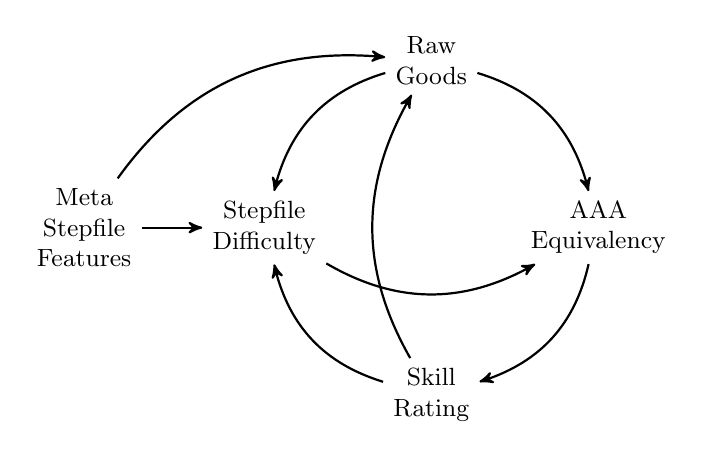
\begin{tikzpicture}[->,>=stealth',auto,align=center,node distance=3cm,
					thick,main node/.style={font=\small}]
					
					\node[main node] (1) {Meta\\Stepfile\\Features};
					\node[main node] (2) [right=1.5cm] {Stepfile\\Difficulty};
					\node[main node] (3) [below right of=2] {Skill\\Rating};
					\node[main node] (4) [above right of=2] {Raw\\Goods};
					\node[main node] (5) [above right of=3] {AAA\\Equivalency};
					
					\path[every node/.style={font=\sffamily\small}]
					(1) edge node [left] {} (2)
					(1) edge [bend left] node [right] {} (4)
					(4) edge [bend right] node [right] {} (2)
					(3) edge [bend left] node [right] {} (4)
					(4) edge [bend left] node [right] {} (5)
					(2) edge [bend right] node [right] {} (5)
					(5) edge [bend left] node [right] {} (3)
					(3) edge [bend left] node [right] {} (2);
					    
				\end{tikzpicture}
			}
		\end{subfloat}
		\hspace{10pt}       
		\begin{subfloat}[Proposed State] {
				\centering
				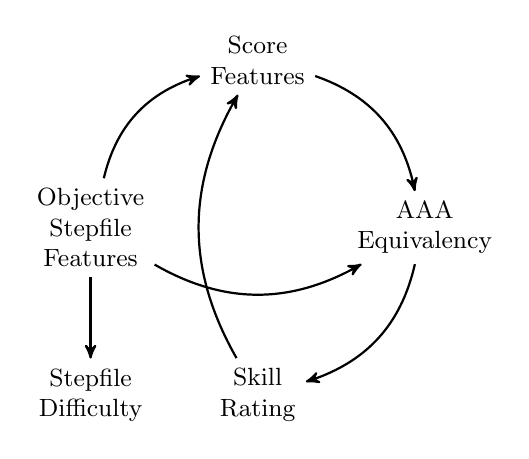
\begin{tikzpicture}[->,>=stealth',auto,align=center,node distance=3cm,
					thick,main node/.style={font=\small}]
					
					\node[main node] (1) {Stepfile\\Difficulty};
					\node[main node] (2) [above=1.5cm] {Objective\\Stepfile\\Features};
					\node[main node] (3) [below right of=2] {Skill\\Rating};
					\node[main node] (4) [above right of=2] {Score\\Features};
					\node[main node] (5) [above right of=3] {AAA\\Equivalency};
					
					\path[every node/.style={font=\sffamily\small}]
					(2) edge node [left] {} (1)
					(2) edge [bend left] node [right] {} (4)
					(3) edge [bend left] node [right] {} (4)
					(4) edge [bend left] node [right] {} (5)
					(2) edge [bend right] node [right] {} (5)
					(5) edge [bend left] node [right] {} (3);
					    
				\end{tikzpicture}
			}       
		\end{subfloat}
		\caption{Dependency graphs differentiating the current and proposed states of skill-based FFR metrics.}
		\label{fig1}
		
	\end{figure}  
\end{center}

From the diagram above, the following changes are recommended:

\begin{itemize}
	\item The stepfile difficulty model will be separated from player performance metrics such as skill rating and raw goods to minimize player subjectivity.
	\item Objective stepfile features will be utilized instead of relying on patterns established by the community to promote consistent terminology.
	\item Raw goods will be replaced with score features to more accurately track player performance.
	\item The AAA equivalency formula will no longer involve stepfile difficulty, but instead will directly incorporate objective stepfile features.
\end{itemize}

Additionally, it is important to note that the Proposed State, as illustrated in Figure \ref{fig1}b, exhibits a circular interdependence between Score Features, AAA Equivalency, and Skill Rating. A well-designed system should be able to:

\begin{itemize}
	\item Accurately assess a player's performance on a stepfile by utilizing score features derived from a predetermined skill rating metric.
	\item Calculate AAA Equivalency without making the assumption of uniform distribution of notes within the stepfile and also take into account performance metrics that are more focused on the player.
	\item Continuously adjust a player's skill rating without distorting their true skill level, which may be influenced by factors such as the number of stepfiles played.
\end{itemize}

The implementation of this study necessitates the development of a framework for training machine learning models using the expectation-maximization algorithm. Within this framework, the models are optimized concerning their corresponding dependent skill-based metrics based on a predetermined convergence criterion. Further details on this approach will be discussed in Section [TODO], with detailed steps for the technical implementation outlined in Section [TODO].

\vspace{2mm}

In Section \ref{sec:stepfile_difficulty}, we aim to establish a clear definition of stepfile difficulty by addressing the inherent subjectivity of this concept. We will examine various existing interpretations and propose a methodology for estimating difficulty based on these definitions. This process includes creating a data stratification strategy to incorporate player feedback from \texttt{\#difficulty-discussion} in FFR's Official Discord channel within our train-test split, identifying a set of objectively defined features that align with specific gameplay properties, and devising a framework for training and evaluating a time series extrinsic regression model. This model will be used to replicate experiments under varying hyperparameter configurations and considered definitions.

\vspace{2mm}

Our definition of AAA equivalency is consistent with the interpretation of the community. However, in Section [TODO], we propose improvements to the current formula by defining an adjusted raw good count concerning features identified for our stepfile difficulty model. Additionally, we introduce precision and recall as performance-indicative metrics within the realm of competitive gameplay by defining the "Boo" judge accuracy label as false positives and the ``Miss" judge accuracy label as false negatives.

\vspace{2mm}

In Section [TODO], we propose a study advocating for the incorporation of outlier detection techniques to eliminate unrepresentative AAA equivalency scores. We also present a framework for adjusting the value of $N$ depending on the number of stepfiles played. Furthermore, we suggest incorporating Seasonal Skill Ratings to contextualize players' abilities beyond their top-performing scores and evaluate their performance in comparison to Skill Ratings.

\section{Stepfile Difficulty Model}
\label{sec:stepfile_difficulty}

\textbf{Plan:}
\begin{itemize}
	\item Untangle objective definitions of difficulty from its inherent subjectivity. Identify that the goal of creating this machine learning model is to maximize the objective representation of difficulty in the overall model.
	      	      
	\item Clarify the definition of difficulty by introducing judge window sizes. Also dissociate processing difficulty from execution difficulty and focus paper on execution. Add visuals:
	      \begin{itemize}
	      	\item Difficulty to FC: 235 ms
	      	\item Difficulty to Clean FC: 201 ms
	      	\item Difficulty to Maximize Score: 153.9 ms
	      	\item Difficulty to Maximize Score under MS based scoring: 117.5 ms
	      	\item Difficulty to AAA: 100 ms
	      	\item Difficulty to AAAA: 34 ms
	      \end{itemize}
	\item Address concerns about inaccurate difficulty measurements current in game and the non-existing idea of "true" difficulty using crowdsourcing papers \href{https://crowdsourcing-class.org/readings/downloads/quality-control/Quality-Management-on-Amazon-Mechanical-Turk.pdf#page4}{here} and \href{https://crowdsourcing-class.org/readings/downloads/ml/EM.pdf}{here}.
	      	      
	      \item{Introduce Contested Difficulty Sheet and define train-test split using KDE estimations of proposed difficulties}
	      	      
	      \item{Introduce objective features VerticalDensity and HorizontalDensity using pen-tapping as an example. Also mention chart augmentation considerations:}
	      \begin{itemize}
	      	\item Mirror: Indirectly accounted in VerticalDensity's definition
	      	\item Offset: Indirectly accounted in preprocessing of FFR's API response.
	      	\item Colors: Categorized under "processing difficulty"; users can alter this.
	      	\item Scroll Speed Mod: Categorized under "processing difficulty"; users can alter this.
	      \end{itemize}
	      	      
	\item Dissociate local features from global features. Song length is a global feature, subsequence extraction is a local feature. Mention how ensembling works with the consideration of "difficulty spikes" in many charts.
	      	      
	\item Introduce model architecture and implementation. Consider regressing over the target variable transformations of difficulty due to domain knowledge of difficulty.
	      	      
	\item Run experiments with proposed model, share results, and identify method to measure the quality of the predictions.
	      	      
	\item Extend proposed model to account for uprated and downrated stepfiles, run experiments and compare model performance with already tracked uprated scores.
	      	          
\end{itemize}

\vspace{2mm}


% In addition to issues mentioned earlier in this report, the evolution of FFR's stepfile difficulty measurement demonstrates the varying perspectives on what constitutes a challenging stepfile. A notable factor contributing to this lack of a consensus is the absence of standardized criteria for determining difficulty. This section aims to establish such standards in order to establish a more reliable and trusted model for evaluating stepfile difficulty, by examining the Contested Difficulties spreadsheet and identifying the difficulty values that hold the most consensus within the FFR community.

\subsection{Contested Difficulty Spreadsheet Analysis}

The Contested Difficulty Spreadsheet, managed by \texttt{Zlyice}, is a collaborative Google Sheets document utilized for tracking proposed changes to stepfile difficulty measurements based on input from users. It is presumed that the individual suggesting a difficulty measurement possesses a degree of knowledge regarding the factors that warrant such a rating for the stepfile. While it must be acknowledged that all proposed measurements are inherently vulnerable to volunteer bias, the process of crowd-sourcing these partial inputs serves to reduce the impact of individual bias on any given stepfile. This approach aims to align the definition of difficulty with the perspectives of the vocal minority within the wider community.

\vspace{2mm}


In order to align our model scoring with the prevailing consensus on the quantification of stepfile difficulty within the community, we conduct a thorough analysis of the proposed difficulty levels over the period spanning from 2022 to the present date. This analysis serves as the basis for our development of a train-test split strategy, in which the distribution of proposed difficulties is utilized to allocate our data into appropriately representative training, validation, and test sets.
\section{AAA Equivalency Model}
\label{sec:aaa_equivalency}

Lorem ipsum dolor sit amet, consectetur adipiscing elit. Etiam fermentum sapien a felis mattis fermentum. Nunc laoreet eros in malesuada ultricies. Sed purus libero, blandit vitae convallis eu, lacinia ut justo. Curabitur est mauris, tincidunt in lacinia et, varius nec tortor. Nunc eu turpis feugiat, porta diam non, tincidunt lorem. Sed pulvinar, metus a volutpat malesuada, urna quam tempor nisi, nec cursus urna dolor vitae felis. Pellentesque posuere neque sapien, quis sagittis neque luctus quis. Quisque ullamcorper dignissim suscipit. Maecenas pharetra, nisi a pretium placerat, ante est posuere mauris, nec auctor mi diam in nisl. Pellentesque ligula magna, volutpat sed nunc vitae, auctor gravida arcu. Maecenas sit amet lacus justo.

\vspace{2mm}

In eu finibus purus. Etiam accumsan erat justo, eu efficitur elit faucibus non. In faucibus vitae nisl dapibus ullamcorper. In fermentum leo eu purus rutrum suscipit. Pellentesque dictum efficitur purus, eu consequat metus pretium a. Vivamus feugiat urna ac accumsan suscipit. Praesent pretium sem risus, a congue felis placerat sed. Maecenas in nisi auctor, aliquet tortor ut, posuere justo. Cras lacinia bibendum elit, ut cursus turpis eleifend vitae. Nunc tempus libero quis suscipit scelerisque. Curabitur aliquet tempor facilisis. Suspendisse auctor, arcu non dictum luctus, sem tortor varius lorem, non commodo nibh arcu non elit. Maecenas maximus maximus justo, vitae bibendum orci semper eget.

\vspace{2mm}

Sed pulvinar leo eget nunc placerat, at cursus quam commodo. Vivamus nunc nisl, posuere id nunc ac, vehicula suscipit dui. Vivamus sodales urna felis, eget gravida nunc dignissim vel. Nam sed libero quis elit fermentum rhoncus. Vestibulum vitae libero et lectus ullamcorper congue eu in ex. In id ultricies enim. Integer volutpat nisi a lorem malesuada ultricies. Pellentesque ut commodo nulla. Nulla eu diam id lectus aliquet venenatis at quis ipsum.

\vspace{2mm}

Nulla ac mauris pharetra turpis interdum faucibus. Sed aliquam tellus ac finibus rutrum. Integer non vulputate sapien. Duis ullamcorper, felis non hendrerit interdum, ex lorem varius mauris, non consectetur eros tellus et ipsum. Nunc scelerisque turpis eu ullamcorper dictum. Cras ligula libero, pellentesque et pretium sed, tristique eget augue. Curabitur magna lectus, aliquam nec ullamcorper a, finibus pulvinar odio. Maecenas dictum, nisl et ornare porttitor, tortor metus molestie massa, ut porta nisi leo non velit. Maecenas quis rhoncus urna. Praesent a lacus vitae erat sagittis facilisis ac ac risus.

\vspace{2mm}

Quisque dapibus semper semper. Phasellus dignissim fringilla mollis. Duis volutpat lacus eget fringilla pretium. Phasellus ut orci non justo viverra aliquet sed at risus. Nulla eu tellus tincidunt, ultrices lectus vitae, tincidunt nibh. Vestibulum ante ipsum primis in faucibus orci luctus et ultrices posuere cubilia curae; Nullam sem orci, fringilla sed nisi et, rhoncus sollicitudin odio. Nam sodales tortor ante, sit amet porttitor ipsum cursus id. Maecenas dapibus mauris nunc, ut placerat dui volutpat vitae. Donec viverra nulla nec libero iaculis mollis. Nullam viverra sit amet felis eu condimentum. In et tempor nibh. Phasellus interdum nibh ornare, scelerisque elit ac, fringilla arcu. Nullam rutrum vestibulum sollicitudin. Proin sem ante, tincidunt et nisi et, ultricies vulputate purus.

\section{Player Skill Rating Model}
\label{sec:player_skill_rating}

Lorem ipsum dolor sit amet, consectetur adipiscing elit. Etiam fermentum sapien a felis mattis fermentum. Nunc laoreet eros in malesuada ultricies. Sed purus libero, blandit vitae convallis eu, lacinia ut justo. Curabitur est mauris, tincidunt in lacinia et, varius nec tortor. Nunc eu turpis feugiat, porta diam non, tincidunt lorem. Sed pulvinar, metus a volutpat malesuada, urna quam tempor nisi, nec cursus urna dolor vitae felis. Pellentesque posuere neque sapien, quis sagittis neque luctus quis. Quisque ullamcorper dignissim suscipit. Maecenas pharetra, nisi a pretium placerat, ante est posuere mauris, nec auctor mi diam in nisl. Pellentesque ligula magna, volutpat sed nunc vitae, auctor gravida arcu. Maecenas sit amet lacus justo.

\vspace{2mm}

In eu finibus purus. Etiam accumsan erat justo, eu efficitur elit faucibus non. In faucibus vitae nisl dapibus ullamcorper. In fermentum leo eu purus rutrum suscipit. Pellentesque dictum efficitur purus, eu consequat metus pretium a. Vivamus feugiat urna ac accumsan suscipit. Praesent pretium sem risus, a congue felis placerat sed. Maecenas in nisi auctor, aliquet tortor ut, posuere justo. Cras lacinia bibendum elit, ut cursus turpis eleifend vitae. Nunc tempus libero quis suscipit scelerisque. Curabitur aliquet tempor facilisis. Suspendisse auctor, arcu non dictum luctus, sem tortor varius lorem, non commodo nibh arcu non elit. Maecenas maximus maximus justo, vitae bibendum orci semper eget.

\vspace{2mm}

Sed pulvinar leo eget nunc placerat, at cursus quam commodo. Vivamus nunc nisl, posuere id nunc ac, vehicula suscipit dui. Vivamus sodales urna felis, eget gravida nunc dignissim vel. Nam sed libero quis elit fermentum rhoncus. Vestibulum vitae libero et lectus ullamcorper congue eu in ex. In id ultricies enim. Integer volutpat nisi a lorem malesuada ultricies. Pellentesque ut commodo nulla. Nulla eu diam id lectus aliquet venenatis at quis ipsum.

\vspace{2mm}

Nulla ac mauris pharetra turpis interdum faucibus. Sed aliquam tellus ac finibus rutrum. Integer non vulputate sapien. Duis ullamcorper, felis non hendrerit interdum, ex lorem varius mauris, non consectetur eros tellus et ipsum. Nunc scelerisque turpis eu ullamcorper dictum. Cras ligula libero, pellentesque et pretium sed, tristique eget augue. Curabitur magna lectus, aliquam nec ullamcorper a, finibus pulvinar odio. Maecenas dictum, nisl et ornare porttitor, tortor metus molestie massa, ut porta nisi leo non velit. Maecenas quis rhoncus urna. Praesent a lacus vitae erat sagittis facilisis ac ac risus.

\vspace{2mm}

Quisque dapibus semper semper. Phasellus dignissim fringilla mollis. Duis volutpat lacus eget fringilla pretium. Phasellus ut orci non justo viverra aliquet sed at risus. Nulla eu tellus tincidunt, ultrices lectus vitae, tincidunt nibh. Vestibulum ante ipsum primis in faucibus orci luctus et ultrices posuere cubilia curae; Nullam sem orci, fringilla sed nisi et, rhoncus sollicitudin odio. Nam sodales tortor ante, sit amet porttitor ipsum cursus id. Maecenas dapibus mauris nunc, ut placerat dui volutpat vitae. Donec viverra nulla nec libero iaculis mollis. Nullam viverra sit amet felis eu condimentum. In et tempor nibh. Phasellus interdum nibh ornare, scelerisque elit ac, fringilla arcu. Nullam rutrum vestibulum sollicitudin. Proin sem ante, tincidunt et nisi et, ultricies vulputate purus.

\section{Future Work}
\label{sec:futurework}

Lorem ipsum dolor sit amet, consectetur adipiscing elit. Etiam fermentum sapien a felis mattis fermentum. Nunc laoreet eros in malesuada ultricies. Sed purus libero, blandit vitae convallis eu, lacinia ut justo. Curabitur est mauris, tincidunt in lacinia et, varius nec tortor. Nunc eu turpis feugiat, porta diam non, tincidunt lorem. Sed pulvinar, metus a volutpat malesuada, urna quam tempor nisi, nec cursus urna dolor vitae felis. Pellentesque posuere neque sapien, quis sagittis neque luctus quis. Quisque ullamcorper dignissim suscipit. Maecenas pharetra, nisi a pretium placerat, ante est posuere mauris, nec auctor mi diam in nisl. Pellentesque ligula magna, volutpat sed nunc vitae, auctor gravida arcu. Maecenas sit amet lacus justo.

\vspace{2mm}

In eu finibus purus. Etiam accumsan erat justo, eu efficitur elit faucibus non. In faucibus vitae nisl dapibus ullamcorper. In fermentum leo eu purus rutrum suscipit. Pellentesque dictum efficitur purus, eu consequat metus pretium a. Vivamus feugiat urna ac accumsan suscipit. Praesent pretium sem risus, a congue felis placerat sed. Maecenas in nisi auctor, aliquet tortor ut, posuere justo. Cras lacinia bibendum elit, ut cursus turpis eleifend vitae. Nunc tempus libero quis suscipit scelerisque. Curabitur aliquet tempor facilisis. Suspendisse auctor, arcu non dictum luctus, sem tortor varius lorem, non commodo nibh arcu non elit. Maecenas maximus maximus justo, vitae bibendum orci semper eget.

\vspace{2mm}

Sed pulvinar leo eget nunc placerat, at cursus quam commodo. Vivamus nunc nisl, posuere id nunc ac, vehicula suscipit dui. Vivamus sodales urna felis, eget gravida nunc dignissim vel. Nam sed libero quis elit fermentum rhoncus. Vestibulum vitae libero et lectus ullamcorper congue eu in ex. In id ultricies enim. Integer volutpat nisi a lorem malesuada ultricies. Pellentesque ut commodo nulla. Nulla eu diam id lectus aliquet venenatis at quis ipsum.

\vspace{2mm}

Nulla ac mauris pharetra turpis interdum faucibus. Sed aliquam tellus ac finibus rutrum. Integer non vulputate sapien. Duis ullamcorper, felis non hendrerit interdum, ex lorem varius mauris, non consectetur eros tellus et ipsum. Nunc scelerisque turpis eu ullamcorper dictum. Cras ligula libero, pellentesque et pretium sed, tristique eget augue. Curabitur magna lectus, aliquam nec ullamcorper a, finibus pulvinar odio. Maecenas dictum, nisl et ornare porttitor, tortor metus molestie massa, ut porta nisi leo non velit. Maecenas quis rhoncus urna. Praesent a lacus vitae erat sagittis facilisis ac ac risus.

\vspace{2mm}

Quisque dapibus semper semper. Phasellus dignissim fringilla mollis. Duis volutpat lacus eget fringilla pretium. Phasellus ut orci non justo viverra aliquet sed at risus. Nulla eu tellus tincidunt, ultrices lectus vitae, tincidunt nibh. Vestibulum ante ipsum primis in faucibus orci luctus et ultrices posuere cubilia curae; Nullam sem orci, fringilla sed nisi et, rhoncus sollicitudin odio. Nam sodales tortor ante, sit amet porttitor ipsum cursus id. Maecenas dapibus mauris nunc, ut placerat dui volutpat vitae. Donec viverra nulla nec libero iaculis mollis. Nullam viverra sit amet felis eu condimentum. In et tempor nibh. Phasellus interdum nibh ornare, scelerisque elit ac, fringilla arcu. Nullam rutrum vestibulum sollicitudin. Proin sem ante, tincidunt et nisi et, ultricies vulputate purus.

\section{Technical Implementation}
\label{sec:technical_implementation}

\begin{center}

\scalebox{0.75}{%
\begin{tikzpicture}
\node[inner sep=0pt] (ffr-database) at (0,1.5)
    {
\includegraphics[width=1.5cm]{figures/diagram/mysql.png}};
\node[align = center, below = of ffr-database] [below=0.2cm of ffr-database]
	{\text\,FFR\\ Database};

\node[inner sep=0pt] (ffr-api) at (4,5)
    {
\includegraphics[width=1.5cm]{figures/diagram/php.png}};
\node[align = center, below = of ffr-api] [below=0.2cm of ffr-api]
	{\text\,FFR\\ API};

\node[inner sep=0pt] (acubed-database-sync) at (8,8)
    {
\includegraphics[width=1.5cm]{figures/diagram/github-actions.png}};
\node[align = center, below = of acubed-database-sync] [below=0.2cm of acubed-database-sync]
	{\text\,ACubed\\ Database Sync};

\node[inner sep=0pt] (acubed-database-reset) at (8,5)
    {
\includegraphics[width=1.5cm]{figures/diagram/github-actions.png}};
\node[align = center, below = of acubed-database-reset] [below=0.2cm of acubed-database-reset]
	{\text\,ACubed\\ Database Reset};

    \node[inner sep=0pt] (acubed-database) at (12,5)
    {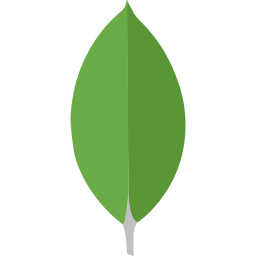
\includegraphics[width=1.5cm]{figures/diagram/mongodb.png}};
\node[align = center, below = of acubed-database] [below=0.2cm of acubed-database]
	{\text\,ACubed\\ Database};
    
    \node[inner sep=0pt] (acubed-codebase) at (12,-1.5)
    {
\includegraphics[width=1.5cm]{figures/diagram/python.png}};
\node[align = center, below = of acubed-codebase] [below=0.2cm of acubed-codebase]
	{\text\,ACubed\\ Codebase};

    \node[inner sep=0pt] (stepfile-difficulty-model) at (8,1.5)
    {
\includegraphics[width=1.5cm]{figures/diagram/difficulty-model.png}};
\node[align = center, below = of stepfile-difficulty-model] [below=0.2cm of stepfile-difficulty-model]
	{\text\,Stepfile Difficulty\\ Model};

    \node[inner sep=0pt] (aaa-equivalency-model) at (8,-1.5)
    {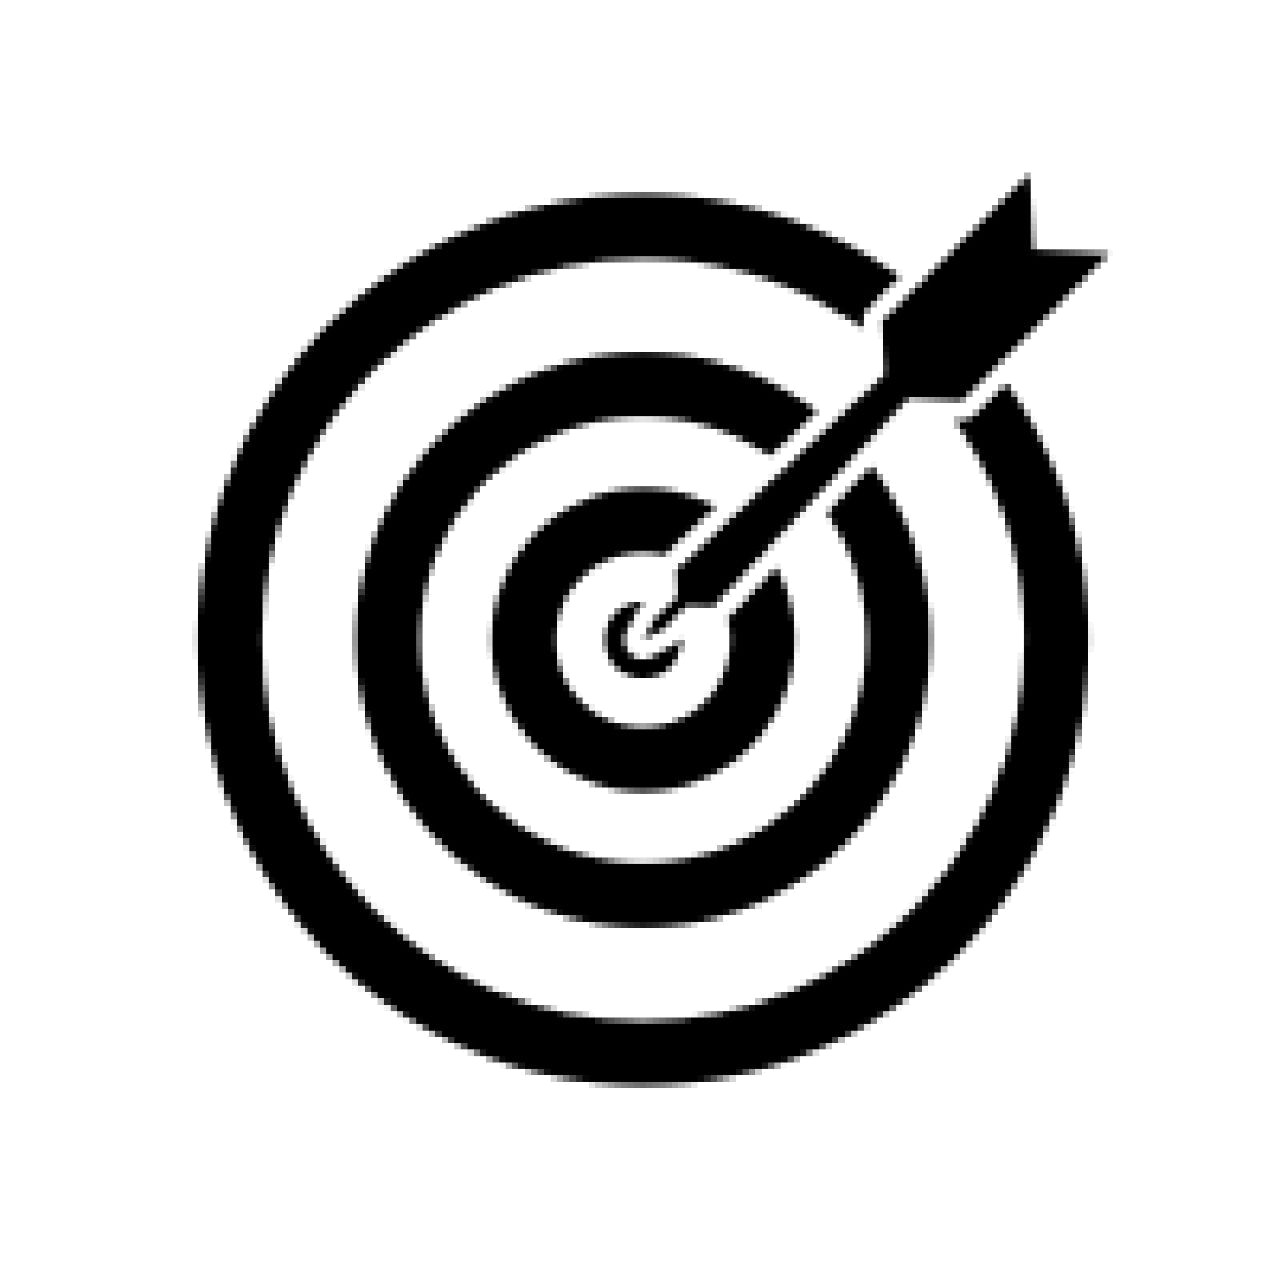
\includegraphics[width=1.5cm]{figures/diagram/aaa-equiv.png}};
\node[align = center, below = of aaa-equivalency-model] [below=0.2cm of aaa-equivalency-model]
	{\text\,AAA Equivalency\\ Model};

    \node[inner sep=0pt] (skill-rating-model) at (8,-4.5)
    {
\includegraphics[width=1.5cm]{figures/diagram/skill-rating.png}};
\node[align = center, below = of skill-rating-model] [below=0.2cm of skill-rating-model]
	{\text\,Skill Rating\\ Model};

    \node[inner sep=0pt] (acubed-api) at (4,1.5)
    {
\includegraphics[width=1.5cm]{figures/diagram/fastapi.png}};
\node[align = center, below = of acubed-api] [below=0.2cm of acubed-api]
	{\text\,ACubed\\ API};

    \node[inner sep=0pt] (rcubed-codebase) at (4,-1.5)
    {
\includegraphics[width=1.5cm]{figures/diagram/rcubed.png}};
\node[align = center, below = of rcubed-codebase] [below=0.2cm of rcubed-codebase]
	{\text\,RCubed\\ Codebase};

    \node[inner sep=0pt] (ffr-engine) at (4,-8)
    {\includegraphics[width=1.5cm]{figures/diagram/air.png}};
\node[align = center, below = of ffr-engine] [below=0.2cm of ffr-engine]
	{\text\,FFR\\ Engine};

    \node[inner sep=0pt] (ffr-website) at (8,-8)
    {\includegraphics[width=1.5cm]{figures/diagram/website.png}};
\node[align = center, below = of ffr-website] [below=0.2cm of ffr-website]
	{\text\,FFR\\ Website};
    
% ffr-database to ffr-api
\draw[-,thick] (0, 2.5) -- (0,5);
\draw[->,thick] (0, 5) -- (3, 5);

% ffr-api to acubed-database-reset
\draw[->,dotted,thick] (5, 5) -- (7, 5);

% ffr-api to acubed-database-sync
\draw[-,thick] (4, 6) -- (4,8);
\draw[->,thick] (4, 8) -- (7, 8);

% acubed-database-sync to acubed-database
\draw[-,thick] (9, 8) -- (12, 8);
\draw[->,thick] (12, 8) -- (12,6);

% acubed-database-sync to acubed-database
\draw[->,dotted,thick] (9, 5) -- (11, 5);

% acubed-database to acubed-codebase
\draw[->,dotted,thick] (12, 3) -- (12, -0.5);

% acubed-codebase to models
\draw[-,dotted,thick] (11, -1.5) -- (10.5, -1.5);
\draw[-,dotted,thick] (10.5, -1.5) -- (10.5, 1.5);
\draw[-,dotted,thick] (10.5, -1.5) -- (10.5, -4.5);
\draw[->,dotted,thick] (10.5, 1.5) -- (9, 1.5);
\draw[->,dotted,thick] (10.5, -1.5) -- (9, -1.5);
\draw[->,dotted,thick] (10.5, -4.5) -- (9, -4.5);

% models to targets
\draw[->,thick] (7, 1.5) -- (5, 1.5);
\draw[->,thick] (7, -1.5) -- (5, -1.5);
\draw[->,thick] (8, -6.5) -- (8, -7);

% acubed-api to ffr-database
\draw[->,dotted,thick] (3, 1.5) -- (1, 1.5);

% ffr-database to ffr-codebase
\draw[-,thick] (0, -0.5) -- (0, -1.5);
\draw[->,thick] (0, -1.5) -- (3, -1.5);

% ffr-codebase to ffr-engine
\draw[->,thick] (4, -3.5) -- (4, -7);

% ffr-engine to ffr-website
\draw[->,thick] (5, -8) -- (7, -8);


\end{tikzpicture}
}
\end{center}

Lorem ipsum dolor sit amet, consectetur adipiscing elit. Etiam fermentum sapien a felis mattis fermentum. Nunc laoreet eros in malesuada ultricies. Sed purus libero, blandit vitae convallis eu, lacinia ut justo. Curabitur est mauris, tincidunt in lacinia et, varius nec tortor. Nunc eu turpis feugiat, porta diam non, tincidunt lorem. Sed pulvinar, metus a volutpat malesuada, urna quam tempor nisi, nec cursus urna dolor vitae felis. Pellentesque posuere neque sapien, quis sagittis neque luctus quis. Quisque ullamcorper dignissim suscipit. Maecenas pharetra, nisi a pretium placerat, ante est posuere mauris, nec auctor mi diam in nisl. Pellentesque ligula magna, volutpat sed nunc vitae, auctor gravida arcu. Maecenas sit amet lacus justo.

\vspace{2mm}

In eu finibus purus. Etiam accumsan erat justo, eu efficitur elit faucibus non. In faucibus vitae nisl dapibus ullamcorper. In fermentum leo eu purus rutrum suscipit. Pellentesque dictum efficitur purus, eu consequat metus pretium a. Vivamus feugiat urna ac accumsan suscipit. Praesent pretium sem risus, a congue felis placerat sed. Maecenas in nisi auctor, aliquet tortor ut, posuere justo. Cras lacinia bibendum elit, ut cursus turpis eleifend vitae. Nunc tempus libero quis suscipit scelerisque. Curabitur aliquet tempor facilisis. Suspendisse auctor, arcu non dictum luctus, sem tortor varius lorem, non commodo nibh arcu non elit. Maecenas maximus maximus justo, vitae bibendum orci semper eget.

\vspace{2mm}

Sed pulvinar leo eget nunc placerat, at cursus quam commodo. Vivamus nunc nisl, posuere id nunc ac, vehicula suscipit dui. Vivamus sodales urna felis, eget gravida nunc dignissim vel. Nam sed libero quis elit fermentum rhoncus. Vestibulum vitae libero et lectus ullamcorper congue eu in ex. In id ultricies enim. Integer volutpat nisi a lorem malesuada ultricies. Pellentesque ut commodo nulla. Nulla eu diam id lectus aliquet venenatis at quis ipsum.

\vspace{2mm}

Nulla ac mauris pharetra turpis interdum faucibus. Sed aliquam tellus ac finibus rutrum. Integer non vulputate sapien. Duis ullamcorper, felis non hendrerit interdum, ex lorem varius mauris, non consectetur eros tellus et ipsum. Nunc scelerisque turpis eu ullamcorper dictum. Cras ligula libero, pellentesque et pretium sed, tristique eget augue. Curabitur magna lectus, aliquam nec ullamcorper a, finibus pulvinar odio. Maecenas dictum, nisl et ornare porttitor, tortor metus molestie massa, ut porta nisi leo non velit. Maecenas quis rhoncus urna. Praesent a lacus vitae erat sagittis facilisis ac ac risus.

\vspace{2mm}

Quisque dapibus semper semper. Phasellus dignissim fringilla mollis. Duis volutpat lacus eget fringilla pretium. Phasellus ut orci non justo viverra aliquet sed at risus. Nulla eu tellus tincidunt, ultrices lectus vitae, tincidunt nibh. Vestibulum ante ipsum primis in faucibus orci luctus et ultrices posuere cubilia curae; Nullam sem orci, fringilla sed nisi et, rhoncus sollicitudin odio. Nam sodales tortor ante, sit amet porttitor ipsum cursus id. Maecenas dapibus mauris nunc, ut placerat dui volutpat vitae. Donec viverra nulla nec libero iaculis mollis. Nullam viverra sit amet felis eu condimentum. In et tempor nibh. Phasellus interdum nibh ornare, scelerisque elit ac, fringilla arcu. Nullam rutrum vestibulum sollicitudin. Proin sem ante, tincidunt et nisi et, ultricies vulputate purus.

\section{Conclusion and Acknowledgements}
\label{sec:conclusion}
Lorem ipsum dolor sit amet, consectetur adipiscing elit. Etiam fermentum sapien a felis mattis fermentum. Nunc laoreet eros in malesuada ultricies. Sed purus libero, blandit vitae convallis eu, lacinia ut justo. Curabitur est mauris, tincidunt in lacinia et, varius nec tortor. Nunc eu turpis feugiat, porta diam non, tincidunt lorem. Sed pulvinar, metus a volutpat malesuada, urna quam tempor nisi, nec cursus urna dolor vitae felis. Pellentesque posuere neque sapien, quis sagittis neque luctus quis. Quisque ullamcorper dignissim suscipit. Maecenas pharetra, nisi a pretium placerat, ante est posuere mauris, nec auctor mi diam in nisl. Pellentesque ligula magna, volutpat sed nunc vitae, auctor gravida arcu. Maecenas sit amet lacus justo.

\vspace{2mm}

In eu finibus purus. Etiam accumsan erat justo, eu efficitur elit faucibus non. In faucibus vitae nisl dapibus ullamcorper. In fermentum leo eu purus rutrum suscipit. Pellentesque dictum efficitur purus, eu consequat metus pretium a. Vivamus feugiat urna ac accumsan suscipit. Praesent pretium sem risus, a congue felis placerat sed. Maecenas in nisi auctor, aliquet tortor ut, posuere justo. Cras lacinia bibendum elit, ut cursus turpis eleifend vitae. Nunc tempus libero quis suscipit scelerisque. Curabitur aliquet tempor facilisis. Suspendisse auctor, arcu non dictum luctus, sem tortor varius lorem, non commodo nibh arcu non elit. Maecenas maximus maximus justo, vitae bibendum orci semper eget.

\vspace{2mm}

Sed pulvinar leo eget nunc placerat, at cursus quam commodo. Vivamus nunc nisl, posuere id nunc ac, vehicula suscipit dui. Vivamus sodales urna felis, eget gravida nunc dignissim vel. Nam sed libero quis elit fermentum rhoncus. Vestibulum vitae libero et lectus ullamcorper congue eu in ex. In id ultricies enim. Integer volutpat nisi a lorem malesuada ultricies. Pellentesque ut commodo nulla. Nulla eu diam id lectus aliquet venenatis at quis ipsum.

\vspace{2mm}

Nulla ac mauris pharetra turpis interdum faucibus. Sed aliquam tellus ac finibus rutrum. Integer non vulputate sapien. Duis ullamcorper, felis non hendrerit interdum, ex lorem varius mauris, non consectetur eros tellus et ipsum. Nunc scelerisque turpis eu ullamcorper dictum. Cras ligula libero, pellentesque et pretium sed, tristique eget augue. Curabitur magna lectus, aliquam nec ullamcorper a, finibus pulvinar odio. Maecenas dictum, nisl et ornare porttitor, tortor metus molestie massa, ut porta nisi leo non velit. Maecenas quis rhoncus urna. Praesent a lacus vitae erat sagittis facilisis ac ac risus.

\vspace{2mm}

Quisque dapibus semper semper. Phasellus dignissim fringilla mollis. Duis volutpat lacus eget fringilla pretium. Phasellus ut orci non justo viverra aliquet sed at risus. Nulla eu tellus tincidunt, ultrices lectus vitae, tincidunt nibh. Vestibulum ante ipsum primis in faucibus orci luctus et ultrices posuere cubilia curae; Nullam sem orci, fringilla sed nisi et, rhoncus sollicitudin odio. Nam sodales tortor ante, sit amet porttitor ipsum cursus id. Maecenas dapibus mauris nunc, ut placerat dui volutpat vitae. Donec viverra nulla nec libero iaculis mollis. Nullam viverra sit amet felis eu condimentum. In et tempor nibh. Phasellus interdum nibh ornare, scelerisque elit ac, fringilla arcu. Nullam rutrum vestibulum sollicitudin. Proin sem ante, tincidunt et nisi et, ultricies vulputate purus.

\clearpage

%----------------------------------------------------------------------------------------
%	Appendix
%----------------------------------------------------------------------------------------
\appendix

\section{Appendix}
\label{sec:appendix}
Lorem ipsum dolor sit amet, consectetur adipiscing elit. Etiam fermentum sapien a felis mattis fermentum. Nunc laoreet eros in malesuada ultricies. Sed purus libero, blandit vitae convallis eu, lacinia ut justo. Curabitur est mauris, tincidunt in lacinia et, varius nec tortor. Nunc eu turpis feugiat, porta diam non, tincidunt lorem. Sed pulvinar, metus a volutpat malesuada, urna quam tempor nisi, nec cursus urna dolor vitae felis. Pellentesque posuere neque sapien, quis sagittis neque luctus quis. Quisque ullamcorper dignissim suscipit. Maecenas pharetra, nisi a pretium placerat, ante est posuere mauris, nec auctor mi diam in nisl. Pellentesque ligula magna, volutpat sed nunc vitae, auctor gravida arcu. Maecenas sit amet lacus justo.

\vspace{2mm}

In eu finibus purus. Etiam accumsan erat justo, eu efficitur elit faucibus non. In faucibus vitae nisl dapibus ullamcorper. In fermentum leo eu purus rutrum suscipit. Pellentesque dictum efficitur purus, eu consequat metus pretium a. Vivamus feugiat urna ac accumsan suscipit. Praesent pretium sem risus, a congue felis placerat sed. Maecenas in nisi auctor, aliquet tortor ut, posuere justo. Cras lacinia bibendum elit, ut cursus turpis eleifend vitae. Nunc tempus libero quis suscipit scelerisque. Curabitur aliquet tempor facilisis. Suspendisse auctor, arcu non dictum luctus, sem tortor varius lorem, non commodo nibh arcu non elit. Maecenas maximus maximus justo, vitae bibendum orci semper eget.

\vspace{2mm}

Sed pulvinar leo eget nunc placerat, at cursus quam commodo. Vivamus nunc nisl, posuere id nunc ac, vehicula suscipit dui. Vivamus sodales urna felis, eget gravida nunc dignissim vel. Nam sed libero quis elit fermentum rhoncus. Vestibulum vitae libero et lectus ullamcorper congue eu in ex. In id ultricies enim. Integer volutpat nisi a lorem malesuada ultricies. Pellentesque ut commodo nulla. Nulla eu diam id lectus aliquet venenatis at quis ipsum.

\vspace{2mm}

Nulla ac mauris pharetra turpis interdum faucibus. Sed aliquam tellus ac finibus rutrum. Integer non vulputate sapien. Duis ullamcorper, felis non hendrerit interdum, ex lorem varius mauris, non consectetur eros tellus et ipsum. Nunc scelerisque turpis eu ullamcorper dictum. Cras ligula libero, pellentesque et pretium sed, tristique eget augue. Curabitur magna lectus, aliquam nec ullamcorper a, finibus pulvinar odio. Maecenas dictum, nisl et ornare porttitor, tortor metus molestie massa, ut porta nisi leo non velit. Maecenas quis rhoncus urna. Praesent a lacus vitae erat sagittis facilisis ac ac risus.

\vspace{2mm}

Quisque dapibus semper semper. Phasellus dignissim fringilla mollis. Duis volutpat lacus eget fringilla pretium. Phasellus ut orci non justo viverra aliquet sed at risus. Nulla eu tellus tincidunt, ultrices lectus vitae, tincidunt nibh. Vestibulum ante ipsum primis in faucibus orci luctus et ultrices posuere cubilia curae; Nullam sem orci, fringilla sed nisi et, rhoncus sollicitudin odio. Nam sodales tortor ante, sit amet porttitor ipsum cursus id. Maecenas dapibus mauris nunc, ut placerat dui volutpat vitae. Donec viverra nulla nec libero iaculis mollis. Nullam viverra sit amet felis eu condimentum. In et tempor nibh. Phasellus interdum nibh ornare, scelerisque elit ac, fringilla arcu. Nullam rutrum vestibulum sollicitudin. Proin sem ante, tincidunt et nisi et, ultricies vulputate purus.


%----------------------------------------------------------------------------------------
%	Bibliography
%----------------------------------------------------------------------------------------

\printbibliography

\end{document}